\section{Hardware}\label{5_1_systemSetup}
\subsection{Components}\label{5_3_systemArchitecture}
%- System architecture of system --> Unity3D, Kinect SDK, Kinectstudio, VGB --> kinect sdk free to use since version X
In the following several hardware components of the system architecture will be described. Each component is necessary for the functionality of the SLS and for the study afterwards. An overview can be seen in figure~\ref{fig:5_3_systemArchitecture}.
% Kinect, Beamer, Screen, Slackline --> Alpidex High Performance

Since the focus of this thesis lies mainly on beginners a short mobile slackline, namely \textit{alpidex POWER-WAVE 2.0}\footnote{\url{http://www.alpidex.com/fitness/slacklines/slackline-gestell-in-2-laengen-power-wave-2-0-inklusive-slackline/a-10288/}} was used.
It provides the needed mobility and independency due to its comparatively short length of three meters.
Hence it is possible to set it up indoors as well as move it in different positions with a minimum of effort.
The included slackline is tensed around brackets at both ends of the device.
The middle rail is divided into two parts and needs to be put together.
It is placed in front of the \textit{Microsoft Kinect v2}, which is used as tracking device, like discussed in section~\textit{\nameref{trackingTechnologie}}. The Kinect itself is attached on a \todo{modell} tripod with a height of about \todo{height, hüfthöhe?}.
A \textit{Steambox PC} \todo{footnote specs} served as development device that fulfilled the recommended specs of the Kinect: \textit{Windows 8, 4 GB Memory, Physical dual-core processor with 3.1 GHz or faster, USB 3.0 Gen-2 controller, Graphics card supporting DirectX 11}. As visual output device a projector \todo{modell} with a resolution of 1920x1080 was attached on a traverse system.
The interface was visualized on a projector screen with a size of \todo{2x3 m} to give the user a more immersive feeling.

\todo{vlt eher bild vom gesamten setup hier rein?}
\begin{figure}[htb]
	\centering
	\begin{minipage}[t]{1\linewidth}
		\centering
		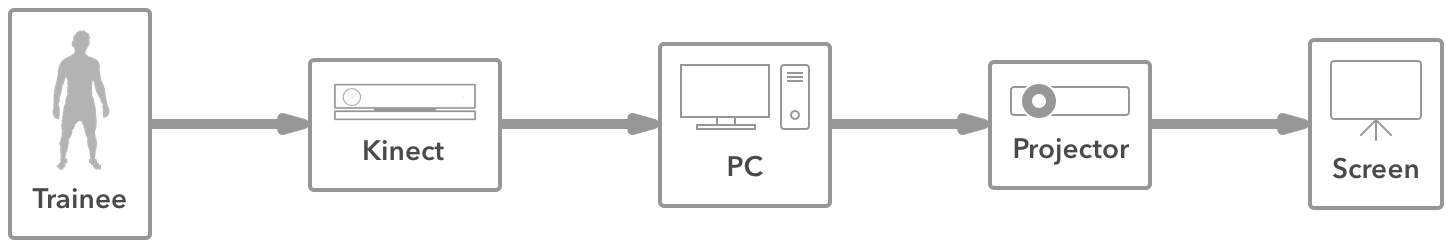
\includegraphics[width=1\linewidth]{Pictures/5_3_systemArchitecture}
		\caption{System overview}
		\label{fig:5_3_systemArchitecture}
	\end{minipage}
\end{figure}

\begin{comment}
\begin{figure}[htb]
	\centering
	\begin{minipage}[t]{1\linewidth}
		\centering
		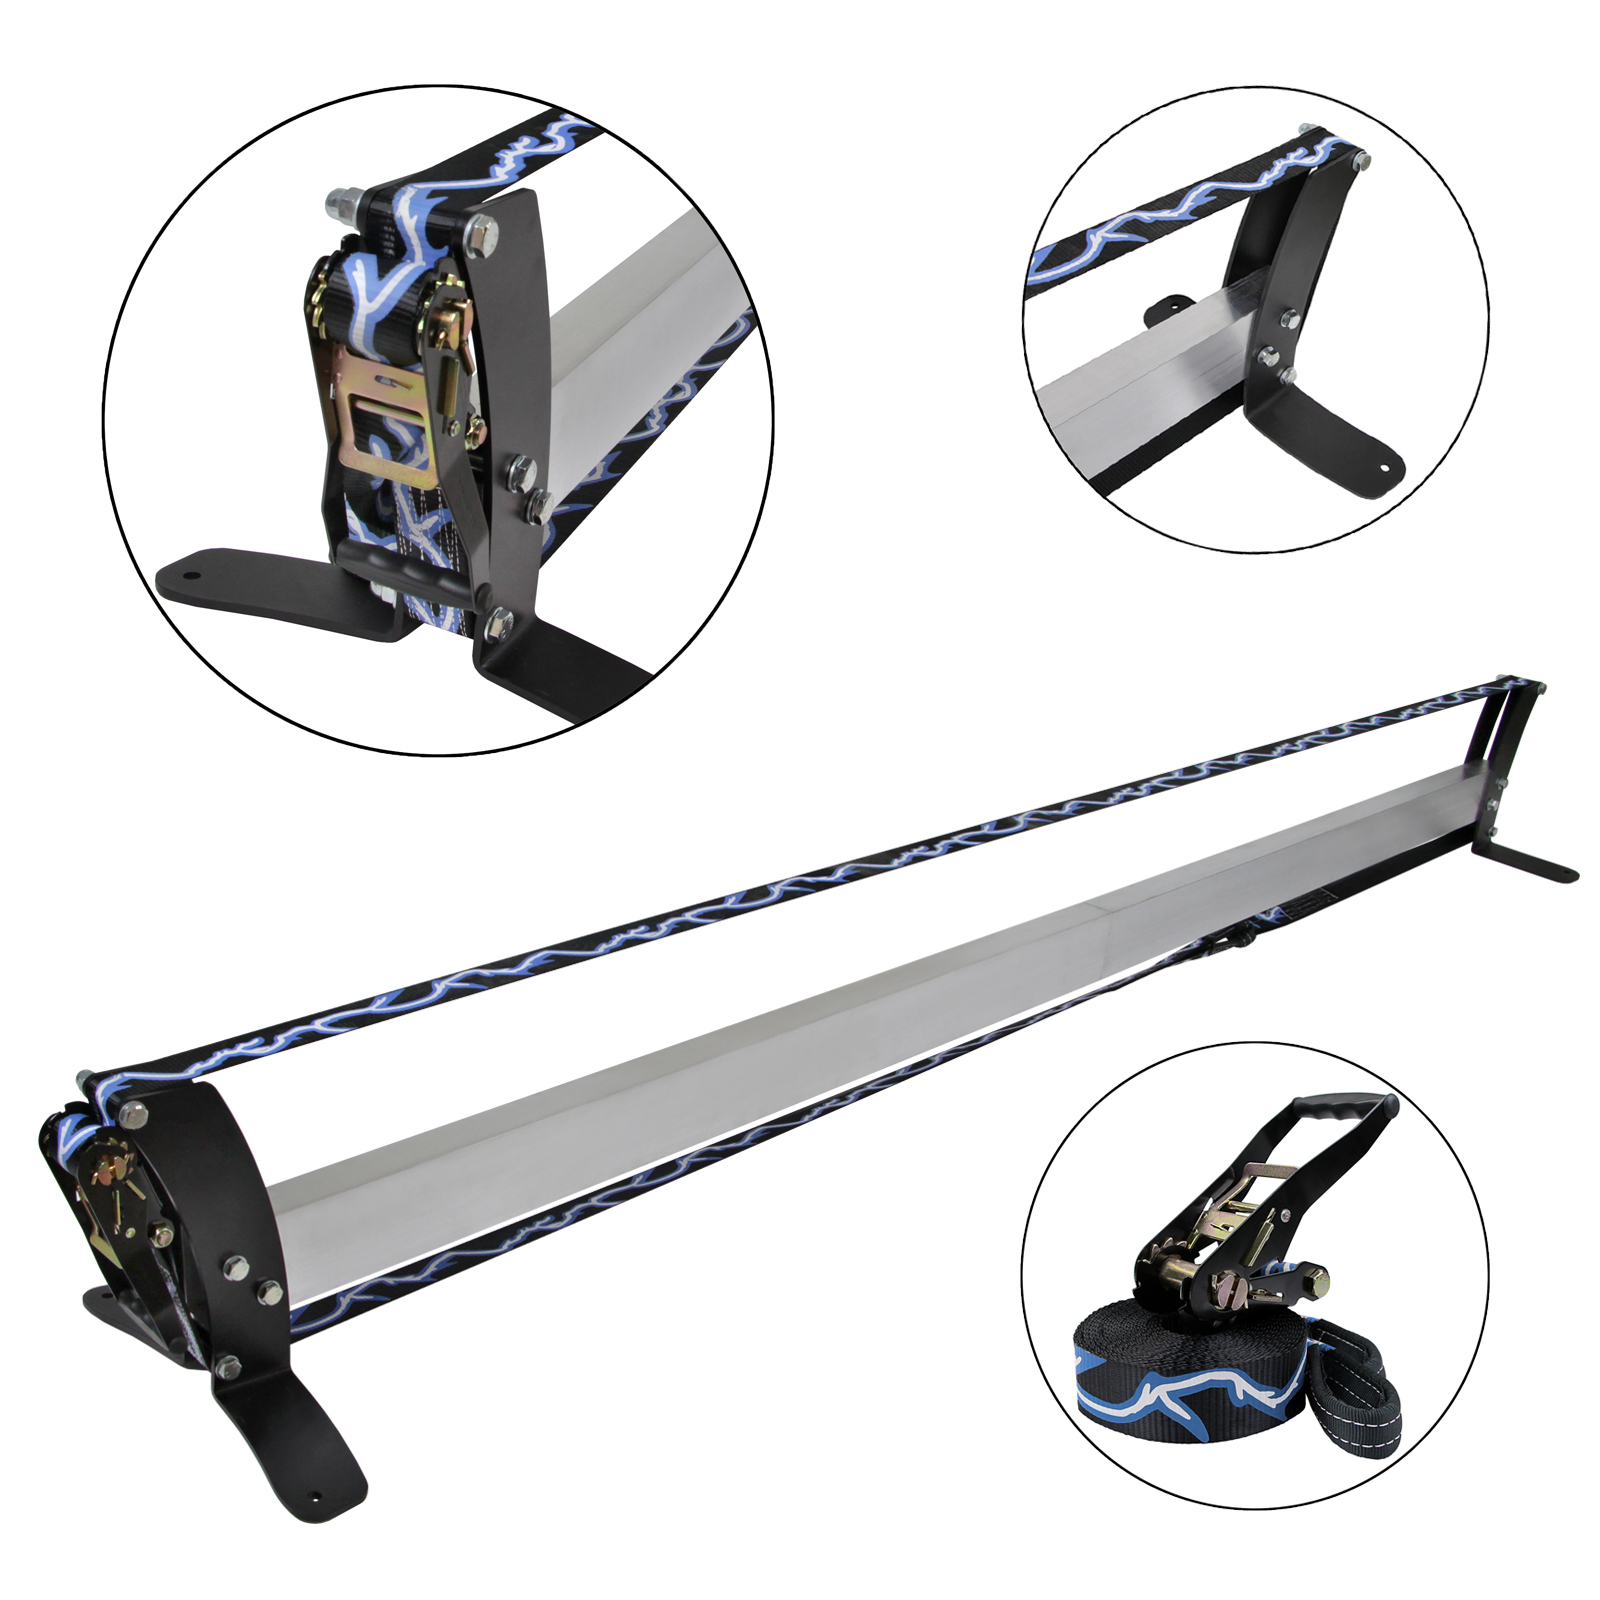
\includegraphics[width=0.44\linewidth]{Pictures/3_2_mobileSlackline}
		\caption{Mobile slackline \textit{alpidex POWER-WAVE 2.0}~\cite{alpidex2017-ms}}
		\label{fig:3_2_mobileSlackline}
	\end{minipage}
\end{figure}
\end{comment}

\subsection{Kinect and Slackline positioning}\label{5_1_technicalFeasibility}
Tracking a person on a slackline with the Kinect is very different from a common situation.
The combination of the slackline range, vibration of the line itself, and unpredictable movements of the user and her balancing actions could lead to imprecise and inaccurate tracking data.
%disturb the tracking performance.
Furthermore, there exists no comparable work about how to track user properly on a slackine with the Kinect.

The major point is to compare different slackline positions (Frontal: 0 Degrees, Diagonal: 45 Degrees, Orthogonal: 90 Degrees) regarding multiple angles and heights of the Kinect on a tripod or traverse system (80 cm, 160 cm, 240 cm).
The testing person was recorded via \textit{KinectStudio}~\footnote{\url{https://developer.microsoft.com/de-de/windows/kinect/tools}}, a tool for recording clips out of the streaming data of the Kinect.
The scenario should clarify how good a person can be tracked on a slackline.
Moreover, which is the best combination of the slackline and Kinect positioning to track user on an entire slackline as well as for study purposes of this thesis.

\subsubsection{Limitations of the Kinect} 
A considerable role plays the angle and tracking range of the Kinects' depth sensor regarding the length of the slackline. Its angle of vision covers in horizontal 70 degrees and in vertical 60 degrees (Figure~\ref{fig:5_1_1_visionAngle}). Since the slackline is about 30 cm off the ground it could lead to tracking problems because. This would result in cropped body parts depending on the users' height. The total tracking range of the sensor covers a range between 0.5 and 4.5 meters, whereas the sweet spot area lies between 1 up to 4 meters~\cite{MicrosoftHIG2014-mh} (Figure~\ref{fig:5_1_1_trackingRange}). The mobile slackline device used in this thesis has a length of three meters and therefore fits entirely within the sweet spot.
\begin{figure}[htb]
	\centering
	\begin{minipage}[t]{0.44\linewidth}
		\centering
		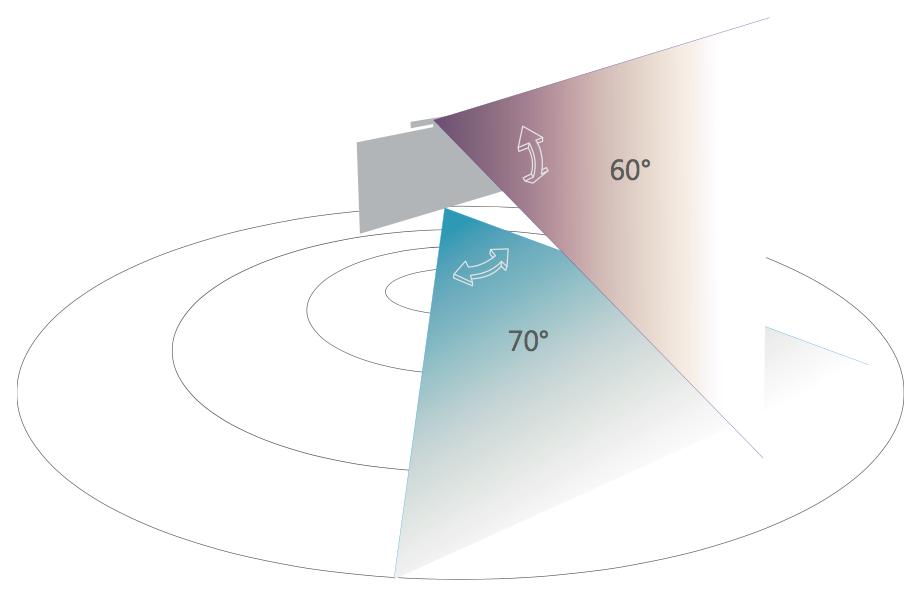
\includegraphics[width=1\linewidth]{Pictures/5_1_1_visionAngle}
		\subcaption{Angle of vision}
		\label{fig:5_1_1_visionAngle}
	\end{minipage}
	\hfill
	\begin{minipage}[t]{0.44\linewidth}
		\centering
		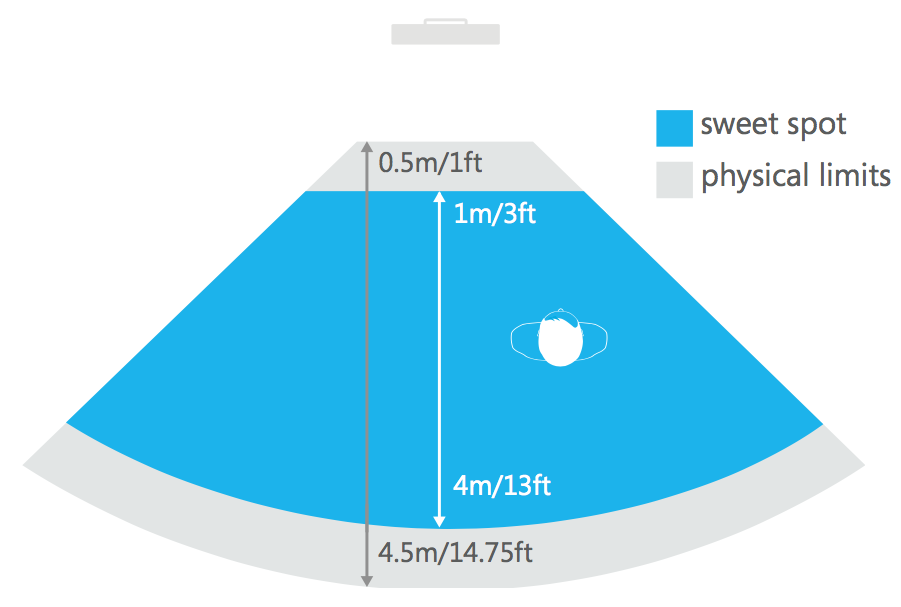
\includegraphics[width=1\linewidth]{Pictures/5_1_1_trackingRange}
		\subcaption{Kinect tracking range}
		\label{fig:5_1_1_trackingRange}
	\end{minipage}
	\caption{Sensor constraints of the Kinect v2~\cite{MicrosoftHIG2014-mh}}
	\label{fig:5_1_1_sensorConstraints}
\end{figure}

%\subsubsection{Testing scenario}

%The test took place in the laboratory of the research group in the \textit{german reasearch center for artificial intelligence}~\footnote{\url{https://www.dfki.de/web/kontakt/dfki-saarbruecken}}. A big advantage of this is the large space to place the slackline easily in different variations. 
%The slackline is placed in three positions to the Kinect: frontal (0 Degree), diagonal (45 Degree) and sideways (90 Degree) \textbf{\todo{(Figure X - 1)}}. Each of this positions is tested regarding three different height levels of the Kinect: 80 cm, 160 cm, and 240 cm. Therefore it was attached on a tripod or traverse system (\textbf{\todo{Figure X - 2}}). At the end nine different combinations are covered to track a user on a slackline, which gives a general overview of the Kinect height to the slackline. The testing person was recorded via \textit{KinectStudio}~\footnote{\url{https://developer.microsoft.com/de-de/windows/kinect/tools}}, a tool for recording clips out of the streaming data of the Kinect.
%In the following the results discuss the feasibility and appropriate tracking positions.

\subsubsection{Best positioning for study purposes}
\todo{sideways und diagonal evtl zusammenfassen}

With a slackline positioned orthogonal (90 Degrees) to the Kinect, the advantage is that the whole body on the slackline is in a constant line within the tracking area. No interference regarding the limits of the tracking range can happen. However, the Kinect had problems to detect the body joints with appropriate accuracy and precision, because of overlapping body parts when standing orthogonal to it (\textbf{\todo{Figure X}}).

Better results have been achieved by placing the slackline diagonal (45 Degrees) to the Kinect. Several body parts will not overlap because the body is more visible to the sensor.
%the frontal and end point of the slackline now differ in the vertical axis, which is unproblematic  \textbf{\todo{(Table X and Figure X)}}. 
%This could even result in a better trackability in matter of the depth field range, since the distance in the front shrinked and is therefore closer to the Kinect depth view. 
But the joints of the arms interfere with other body joints, especially at the end of the line. Also both legs occlude while stepping forwards \textbf{\todo{(Figure X)}}. 
%This results in a relatively bad skeletal tracking and depending on the executed exercise it can lead to detection problems.

Positioning the slackline frontal towards the Kinect resulted in the best user tracking.
The Kinect can see the full body and track the joints without any problems.
However, tracking failures occurred at the starting position of the slackline. This is because the slackline utilises the entire tracking range and therefore the user stands closer to the outermost limit of this range.
~\textbf{\todo{(Figure X)}}.

%Three main height levels were used to show the main differences of the tracking behaviour from the Kinect. It is mounted on a tripod and covers the heights of 0.80, 1.60 and 2.40 meters off the ground. 

Beginning with a height of 2.40 meters the Kinect has a very steep view angle.
%to track the slackers' body on the full range of the slackline. 
Because of this the tracking range shifts more into the front like seen in \textbf{\todo{Figure X}}. If beginning at the starting position on the slackline the slacker reaches hereby immediately the end of the tracking area. Also the further she walks towards the Kinect the more joints will overlap .

With a height between 1.60 and 0.80 meters the body is fully visible in the entire tracking range. The Kinect has a relatively flat view angle and it results in a more homogeneous tracking range (\textbf{\todo{Figure X}}).
%Problems can occur with positioning the Kinect on a lower height. It can lead to cropped body parts like the head or arms at the very end of the slackline.
If the height of the Kinect is about 1.60 m the slackline must be positioned further away from the Kinect to prevent cropped body parts like the head or arms at the very end of the line.

\todo{\textbf{table}}
%The tracking and view is more homogeneous and the angle flatter, which results in the possibility to use the full depth range. With a higher attachment the angle will be too steep, which results in less depth range, as well as more occlusions of body parts can occur.
\rowcolors{2}{tablerowgray}{tablerowgray}
\begin{table}[h!]
\centering
%\arrayrulecolor{white}
\renewcommand{\arraystretch}{1}
\begin{tabular}{ | c | c | c | c | c | c | c | c | }
\hline
\rowcolor{tableheadergray} & \multicolumn{7}{ c| }{\textbf{Slackline Positioning (m)}} \\ 
\rowcolor{tableheadergray} & \multicolumn{2}{ c| }{\textbf{Frontal}} & \multicolumn{2}{ |c| }{\textbf{Diagonal}} & \multicolumn{3}{ |c| }{\textbf{Sideways}}\\
\rowcolor{tableheadergray} \multirow{-3}{*}{\textbf{Kinect Height (m)}} & \textbf{Front} & \textbf{Back} & \textbf{Front} & \textbf{Back} & \textbf{Front} & \textbf{Back} & \textbf{Mid} \\
\hline
2,40 & 1.30 & 4.30 & 1.90 & 3.80 & 3.00 & 3.00 & 2.70 \\
\hline
1.60 & 1.70 & 4.70 & 2.10 & 4.00 & 3.00 & 3.00 & 2.70 \\
\hline
0.80 & 1.30 & 4.30 & 1.90 & 3.80 & 2.60 & 2.60 & 2.10 \\
\hline
\rowcolor{green} 0.80 - 1.20 & 0.00 & 4.00 & - & - & - & - & - \\
\hline
\end{tabular}
\caption{Demographic data and physical activity table}
\label{table:1}
\end{table}

% But since beginner will use the entire slackline range it can be neglected.
The best combination resulted placing the slackline frontal and having a Kinect height of 0.80 up to 1.20 meters. The Kinect can track the entire body with nearly no joint overlap. Since the focus of the study in this thesis lies mainly on beginners, the starting position of the slackline plays an important role. Hence, it is better to move the slackline very close to the Kinect because the very end of the line is not important for the study.
%a little bit of slackline is cropped out of the view but 
With this a higher tracking confidence is possible at the starting position, which is more important in this case \textbf{\todo{(Figure X)}}.
%This results in a relatively bad skeletal tracking and depending on the executed exercise it can lead to detection problems.